\documentclass[preview]{standalone}

\usepackage{pgfplots}
\usepgfplotslibrary{fillbetween}
\usetikzlibrary{patterns}

\pgfplotsset{
  ticks=none,
  samples = 300
}

\begin{document}
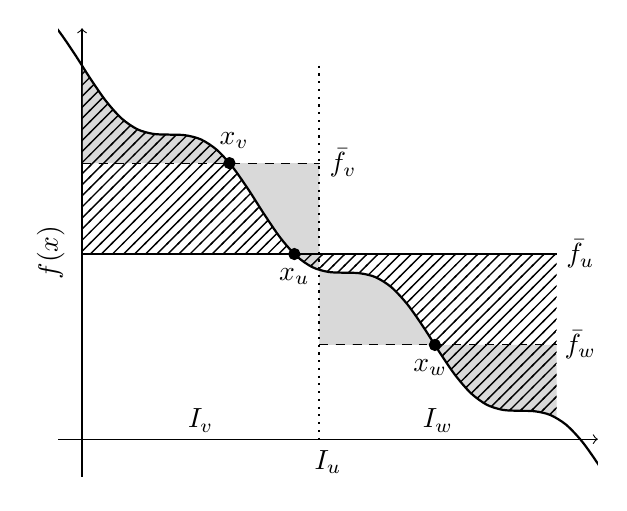
\begin{tikzpicture}
    \tikzset{
        hatch distance/.store in=\hatchdistance,
        hatch distance=10pt,
        hatch thickness/.store in=\hatchthickness,
        hatch thickness=2pt
    }

    \makeatletter
    \pgfdeclarepatternformonly[\hatchdistance,\hatchthickness]{flexible hatch}
    {\pgfqpoint{0pt}{0pt}}
    {\pgfqpoint{\hatchdistance}{\hatchdistance}}
    {\pgfpoint{\hatchdistance-1pt}{\hatchdistance-1pt}}%
    {
        \pgfsetcolor{\tikz@pattern@color}
        \pgfsetlinewidth{\hatchthickness}
        \pgfpathmoveto{\pgfqpoint{0pt}{0pt}}
        \pgfpathlineto{\pgfqpoint{\hatchdistance}{\hatchdistance}}
        \pgfusepath{stroke}
    }


  \begin{axis}[enlargelimits=0.1,ymin=-0.1,ymax=1.1,
    axis lines=middle,
    axis line style={->},
    x label style={at={(axis description cs:0.5,0.08)},anchor=north},
    y label style={at={(axis description cs:0.03,0.5)},rotate=90,anchor=south},
    xlabel={$I_u$},
    ylabel={$f(x)$}
    ]

    \addplot[name path=test,black,smooth,thick]{1.0 - (x + sin(deg(17.0*x))/17.0)};

      \addplot[name path=phat,domain=0.0:1.0,black] {0.49559};
      \addplot[name path=lefthat,domain=0.0:0.5,black,dashed] {0.73892};
      \addplot[name path=righthat,domain=0.5:1.0,black,dashed] {0.252262};
      
      \addplot +[mark=none,black,dotted,thick] coordinates {(0.5, 1) (0.5, 0)};


      \addplot [
      thick,
      color=gray,
      fill=gray,
      fill opacity=0.3
      ]
      fill between[
      of=test and lefthat,
      soft clip={domain=0.0:0.5},
      ];

      \addplot [
      thick,
      color=gray,
      fill=gray,
      fill opacity=0.3
      ]
      fill between[
      of=test and righthat,
      soft clip={domain=0.5:1.0},
      ];

      \addplot [
      pattern=flexible hatch,
      hatch distance=5pt,
      hatch thickness=0.5pt,
      pattern color=black
      ]
      fill between[
      of=test and phat,
      soft clip={domain=0.0:1.0},
      ];
      
      \node at (axis cs: 0.25, 0.05) {$I_v$};
      \node at (axis cs: 0.75, 0.05) {$I_w$};

      \node at (axis cs: 0.55, 0.73892) {$\bar{f}_v$};
      \node at (axis cs: 1.05, 0.49559) {$\bar{f}_u$};
      \node at (axis cs: 1.05, 0.252262) {$\bar{f}_w$};
      
      \addplot[only marks] table {
        0.310647 0.73892
        0.447391 0.49559
        0.743470 0.252262
      };

      \node at (axis cs: 0.320647, 0.79892) {$x_v$};
      \node at (axis cs: 0.447391, 0.43559) {$x_u$};
      \node at (axis cs: 0.733470, 0.192262) {$x_w$};
    \end{axis}
\end{tikzpicture}
\end{document}